\section{Methods}\label{sec:method}

\subsection{Normalization of \ac{dce}-\ac{mri} images}\label{sec:norm}

\begin{figure}
  \centering
  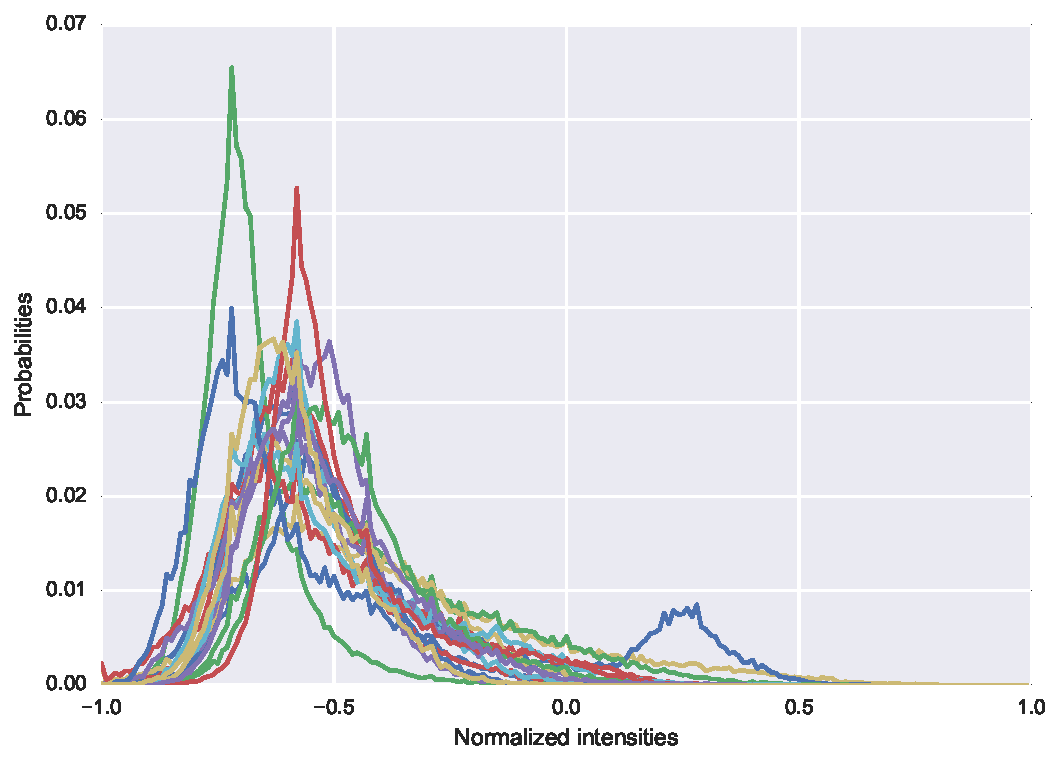
\includegraphics[width=0.7\linewidth]{02_methods/figures/t2w.pdf}
  \caption{\textbf{Illustration of the inter-patient variations in 17
    different patients in \acs*{t2w}-\acs*{mri}, using the \acs*{pdf} representation.}}
  \label{fig:t2w}
\end{figure}

In this work, we propose a method to normalize \ac{dce}-\ac{mri}
prostate data to reduce inter-patient variations, although this method can be applied to any \ac{dce}-\ac{mri} sequences.
In \ac{t2w}-\ac{mri}, these variations are characterized by a shift and a scaling of the intensities as illustrated by the intensity \ac{pdf} in Fig.\,\ref{fig:t2w}.
Therefore, these variations can be corrected using a $z$-score approach,--- i.e., normalizing the data by subtracting the mean and dividing by the standard deviation ---assuming that the data follow a specific distribution~\citep{lemaitre2016normalization}.

\begin{figure*}
  \centering
  \hspace*{\fill}
  \subfigure[]{\label{subfig:pathhist}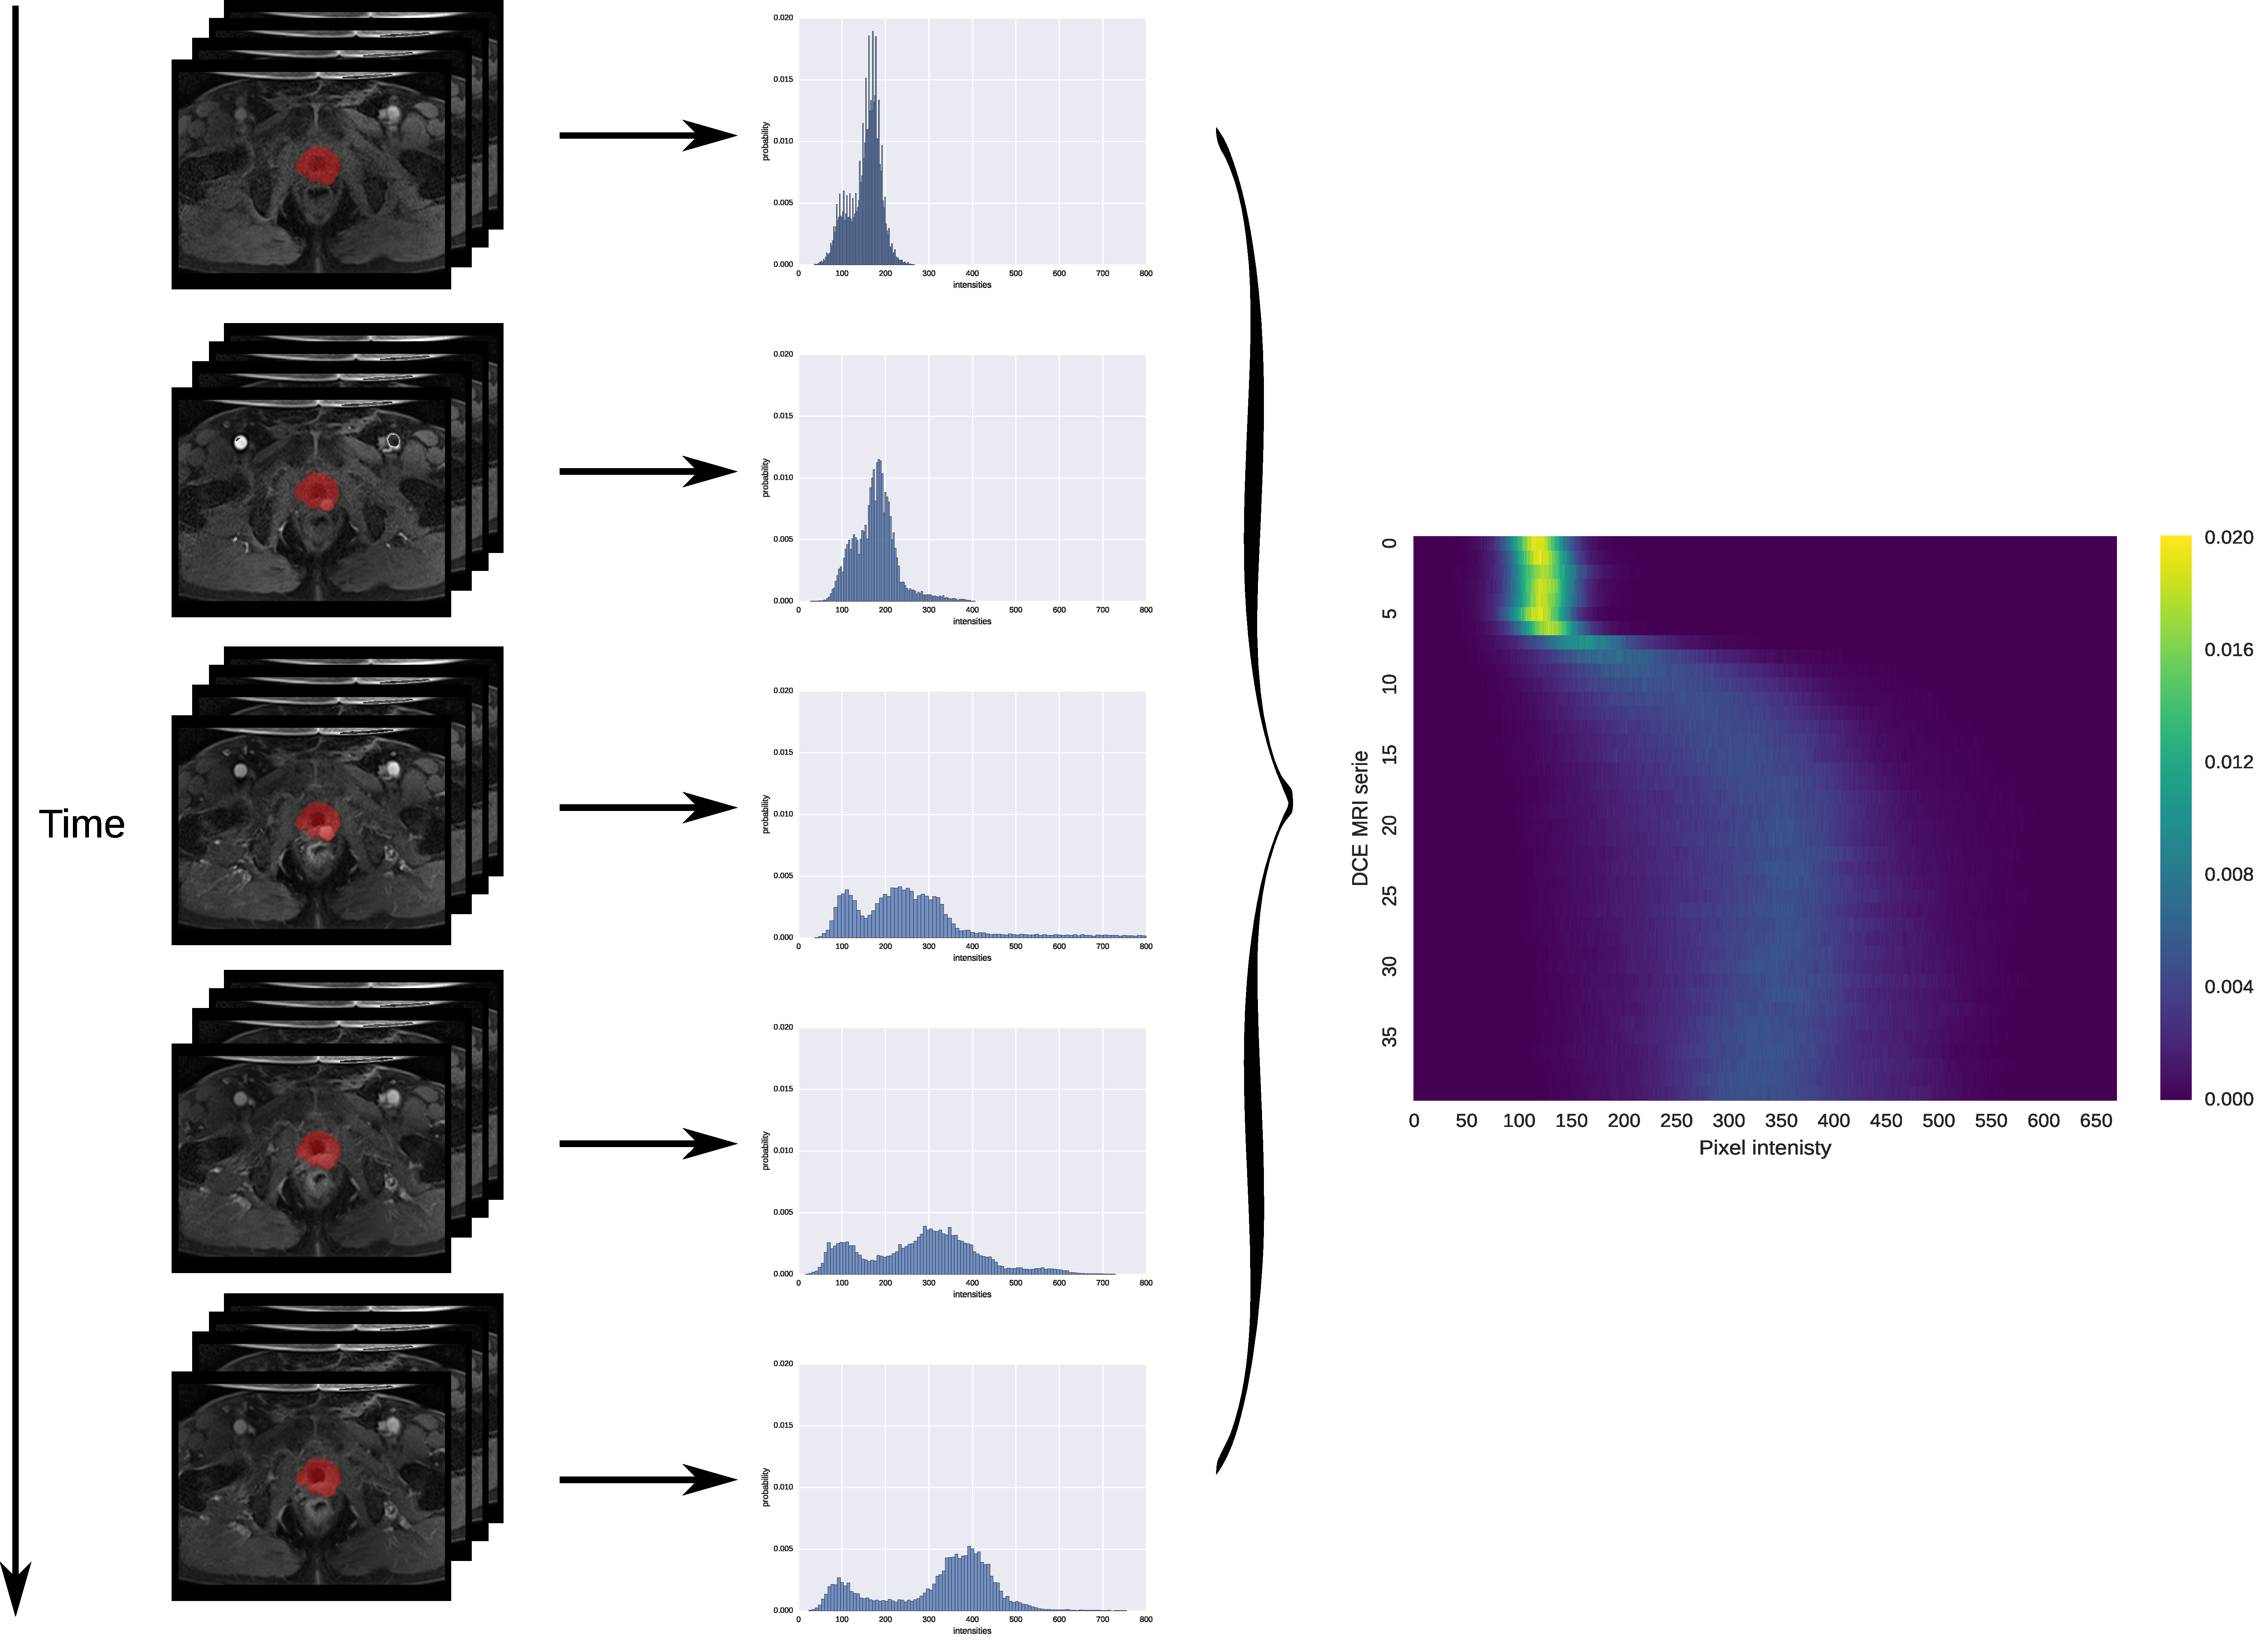
\includegraphics[width=1\textwidth]{02_methods/figures/heatmaprep.pdf}} \hfill
  \hspace*{\fill}
  \\
  \hspace*{\fill}
  \subfigure[\textbf{$I_0$: 117; $t_0$: 6\textsuperscript{th} serie; wider st. dev.}]{\label{subfig:pat1}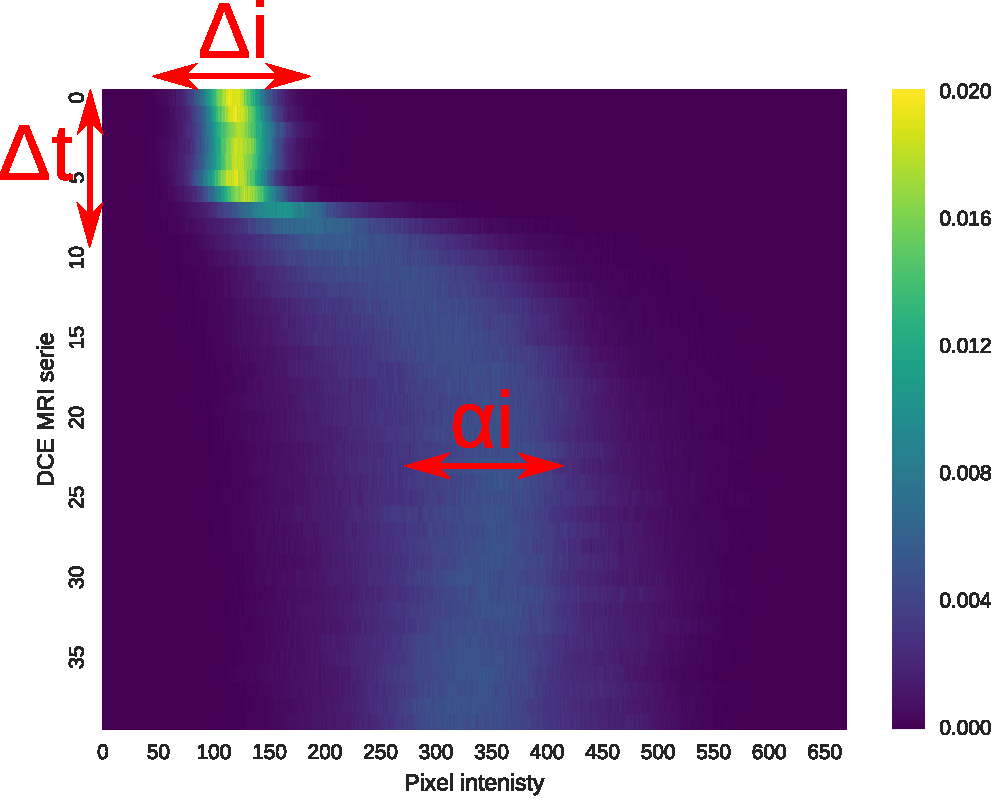
\includegraphics[width=.49\textwidth]{02_methods/figures/pat1_annotated.pdf}} \hfill
  \subfigure[\textbf{$I_0$: 103; $t_0$: 4\textsuperscript{th} serie; narrower std. dev.}]{\label{subfig:pat2}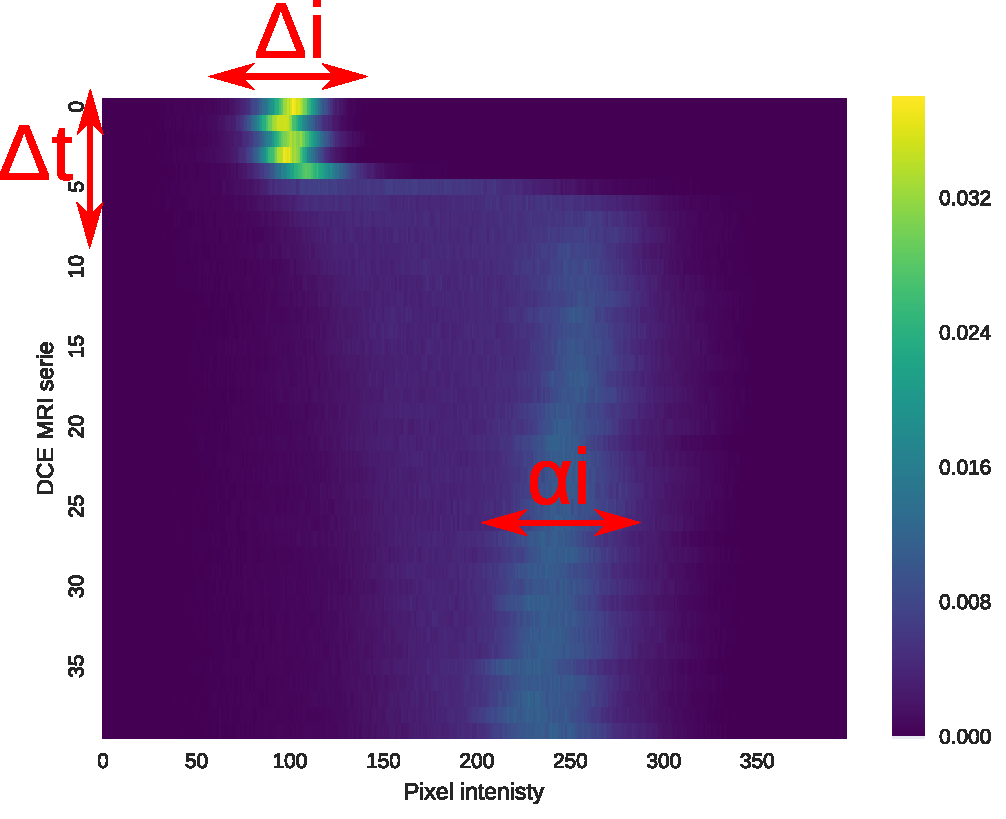
\includegraphics[width=.49\textwidth]{02_methods/figures/pat2_annotated.pdf}} \hfill
  \hspace*{\fill}
  \caption{\subref{subfig:pathhist} Illustration of the heatmap
    representation: all \ac*{pdf}s of the prostate gland are
    concatenated together to build an heatmap;
    \subref{subfig:pat1}-\subref{subfig:pat2} Heatmap of 2 patients
    revealing  the three types of inter-patient variations: intensity shift
    ($\Delta_i$), time shift ($\Delta_t$), and intensity scale
    ($\alpha_i$).}
  \label{fig:heatmap}
\end{figure*}

In \ac{dce}-\ac{mri}, the intensity \ac{pdf} of the prostate gland does not follow a unique type of distribution such as Rician or Gaussian distribution, as shown in Fig.\,\ref{subfig:pathhist}.
Indeed, the inter-patient variations are more complex due to the temporal acquisition.
A better means of observing these variations is to represent the
intensity \ac{pdf} of the prostate gland over time---, requiring
segmentation of the prostate ---using a heatmap representation as shown in Fig.\,\ref{subfig:pathhist}.
By analyzing this heatmap representation across patients (see Fig.\,\ref{subfig:pat2}), the following variations are highlighted:
(i) intensity offsets ($\Delta_i$) of the \ac{pdf} peak,
(ii) a time offset ($\Delta_t$) depending on the contrast agent arrival, and
(iii) a change of scale ($\alpha_i$) related to the signal enhancement.
Therefore, our normalization method should attenuate all of these variations and be performed globally across the different time sequences rather than for each independent sequence.

\subsubsection{Graph-based intensity offsets correction}\label{sec:intoffsets}

\begin{figure}
  \centering
  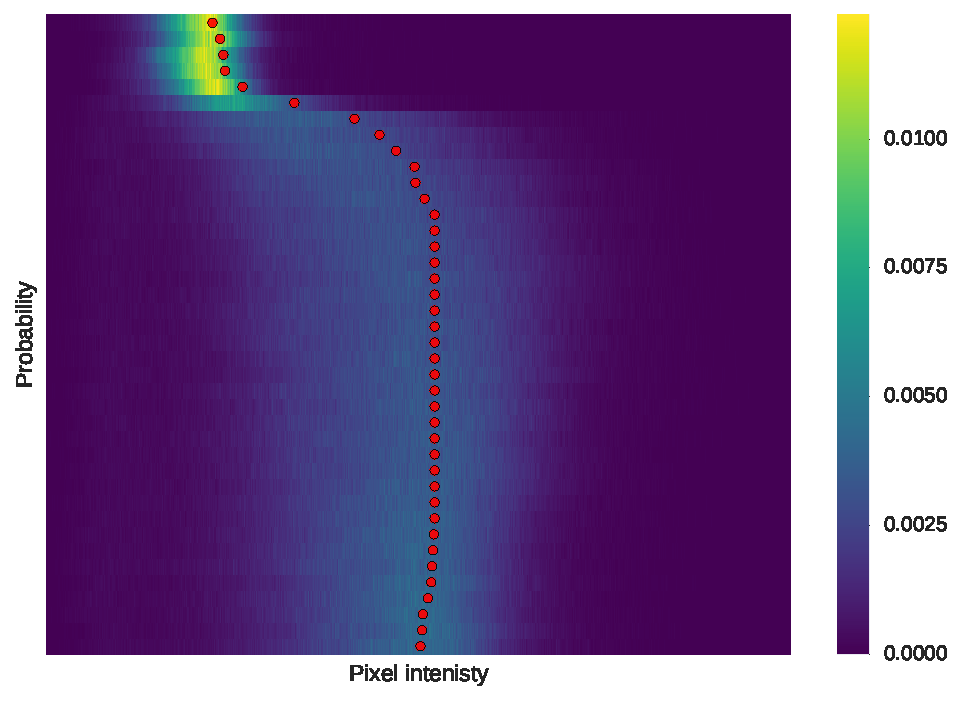
\includegraphics[width=0.7\linewidth]{02_methods/figures/estimator.pdf}
  \caption{Illustration of the estimator found using the shortest-path through the graph.}
  \label{fig:estimator}
\end{figure}

Before standardizing each sequence, the first step of the
normalization process is to cancel the intensity specific at each
patient, which occurs due to the media injection.
As previously mentioned, the intensity \ac{pdf} does not always follow a Rician or a Gaussian distribution over time, in \ac{dce}-\ac{mri}.
Therefore, the mean of these distributions cannot be used as a potential estimate for these offsets.
Additionally, these offsets should be characterized by a smooth transition between series over time.
Thus, this problem is solved using the graph-theory: considering the intensity \ac{pdf} over time as shown in Fig.\,\ref{subfig:pathhist}, the offsets correspond to the boundary splitting, the heatmap into two partitions such that they are as close as possible to the peak of the intensity \ac{pdf} (see Fig.\,\ref{fig:estimator} for an illustration).
Given the heatmap, a directed weighted graph
$\mathcal{G}=(\mathcal{V}, \mathcal{E})$ is built by taking each
bar---, i.e., the probability for a given time and pixel intensity---,
of the heatmap as a node and connecting each pair of bars by an edge.
The edge weight $w_{ij}$ between two nodes $i$ and $j$ corresponds to
two pixels at positions $(x_i, y_i)$ and $(x_j, y_j)$, respectively,
is defined as in Eq.\,\eqref{eq:weight}, as follows:

\begin{equation}
  w_{ij} = \begin{cases}
    \alpha \exp(1 - \frac{H(i)}{\max(H)})       & \text{if } x_j = x_i + 1 \text{ and } y_j = y_i, \\
    (1 - \alpha) \exp(1 - \frac{H(i)}{\max(H)}) & \text{if } x_j = x_i \text{ and } y_j = y_i + 1, \\
    0                                           & \text{otherwise},
  \end{cases}
  \label{eq:weight}
\end{equation}

\noindent where $H$ is the heatmap, and $\alpha$ is a smoothing
parameter controlling for the partitioning.

Therefore, these offsets related to $\Delta_i$ are estimated by finding the shortest-path to cross the graph using Dijkstra's algorithm.
The entry and exiting nodes are set to be the bin with the maximum
probability for the first value in the \ac{dce}-\ac{mri} series and
the bin corresponding to the median value for the last value of the \ac{dce}-\ac{mri} series, respectively.
To ensure a robust estimation of these offsets, the process of finding the shortest-path is repeated by shifting the data and updating the heatmap as well as the graph $\mathcal{G}$.
The procedure is stopped once the offset found does not change.
In general, this process is not repeated more than 3 times.
The parameter $\alpha$ is set to $0.9$, empirically.
Figure~\ref{fig:estimator} illustrates the final estimation of the
offsets, $\Delta_i$ (i.e., red landmark), found for each value of the \ac{dce}-\ac{mri} series.
Therefore, each intensity offset is subtracted for each \ac{dce}-\ac{mri}.

\subsubsection{Time offset and data dispersion correction}

\begin{figure*}
  \centering
  \hspace*{\fill}
  \subfigure[\acs*{rmse} computed for each patient of our dataset.]{\label{fig:rmse}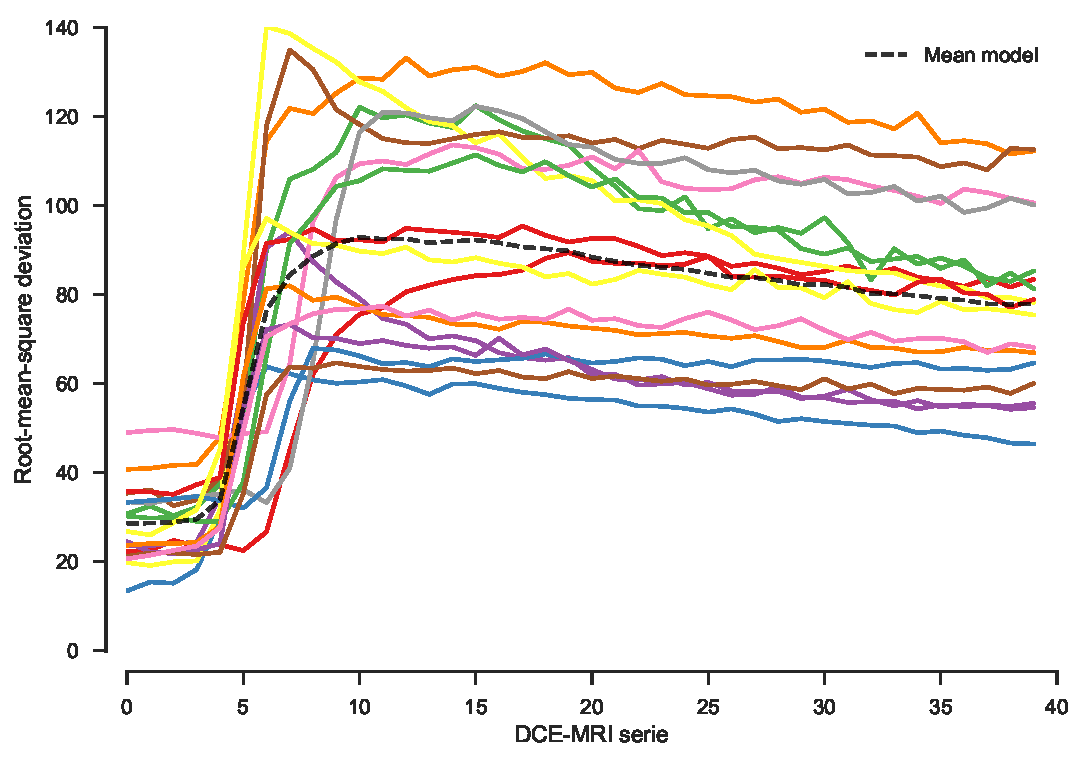
\includegraphics[width=.44\textwidth]{02_methods/figures/rmse.pdf}} \hfill
  \subfigure[\acs*{rmse} after alignment using the curve parametric model.]{\label{fig:rmseal}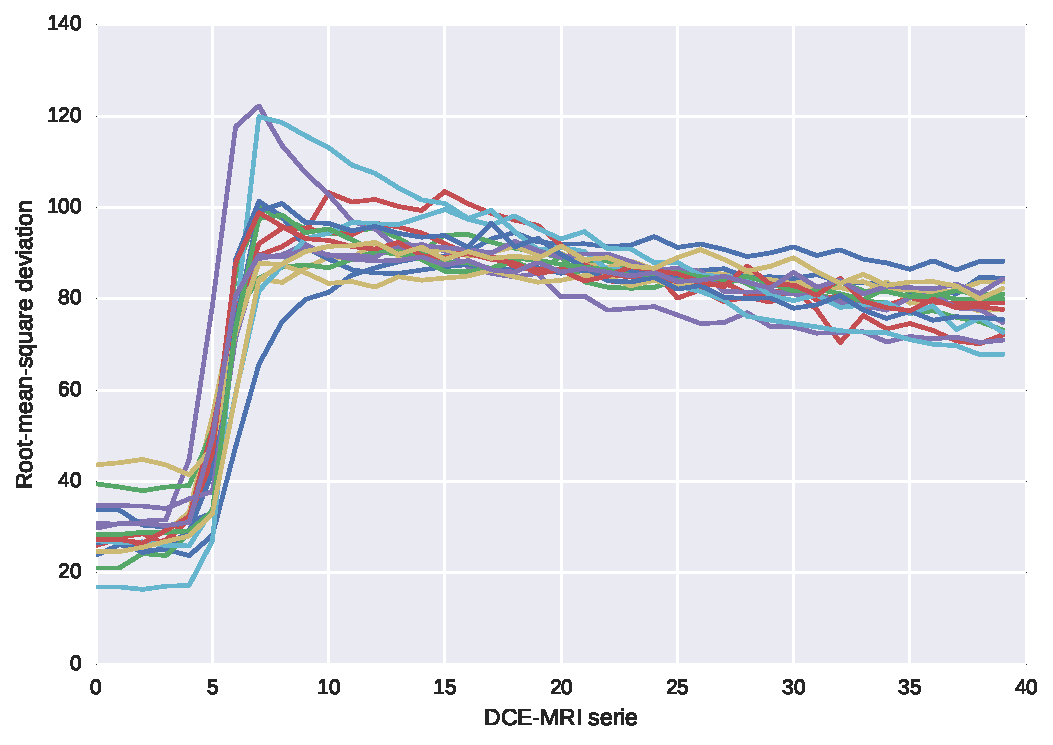
\includegraphics[width=.49\textwidth]{02_methods/figures/rmse_aligned.pdf}}
  \hspace*{\fill}
  \caption{Illustration of the correction of the time offset and the data dispersion.}
  \label{fig:curveal}
\end{figure*}

The next variations to correct are the time offset, $\Delta_t$, and the data dispersion, $\sigma_i$.
By computing the \ac{rmse} of the intensities for each value of the \ac{dce}-\ac{mri} series, one can observe these two variations as shown in Fig.\,\ref{fig:rmse}.
Therefore, to correct these variations, we propose the registration of
each patient \ac{rmse} to a mean model that corresponds to the mean of
all patients' \ac{rmse} values.
The parametric model required to perform the registration is
formulated in Eq.\,\eqref{eq:model}, as follows:

\begin{equation}
  T(\alpha, \tau, f(t)) = \alpha f(t - \tau) ,
  \label{eq:model}
\end{equation}

\noindent where $\alpha$ and $\tau$ are the two parameters handling
the time offset $\Delta_i$ and the global scale $\sigma_i$,
respectively, $f(\cdot)$ is the \ac{rmse} function defined as follows:

\begin{equation}
  f(t) = \sqrt{ \left( \frac{\sum_{n=1}^{N} x(t)_{n}^2}{N}  \right) },
  \label{eq:rmsd}
\end{equation}

\noindent where $x(t)_n$ is the shifted intensity of a sample from a
specific \ac{dce}-\ac{mri} series value at time $t$ from a total number of $N$ samples.

Therefore, the registration problem is equivalent to:

\begin{equation}
  \argmin_{\alpha, \tau} = \sum_{t=1}^{N} \left[ T\left(\alpha, \tau, f(t)\right) - \mu(t) \right]^{2} ,
  \label{eq:cost}
\end{equation}

\noindent where $\mu(\cdot)$ is the mean model and, $N$ is the number
of values in the \ac{dce}-\ac{mri} series.

An illustration of the correction applied to each \ac{rmse} of the patients is shown in Fig.\,\ref{fig:rmseal}.
Once all of these parameters have been determined, the data are shifted and scaled.

The resulting normalized data can be used into two ways: (i) each
normalized signal can be used as a whole to determine if the corresponding voxel is healthy or cancerous or (ii) the normalized data can be fitted using a quantitative method, as presented in the next section.
%However, for the second strategy, this is necessary to apply common intensity offsets such that the data follow a shape as expected by the different quantitative models.
%The set of offsets applied is in fact corresponding to the maximum offsets found in Sect.\,\ref{sec:intoffsets}.

\subsection{Quantification of \ac{dce}-\ac{mri}}\label{sec:stateart}

In this section, we summarize the different methods that have been
used for the quantification of \ac{dce}-\ac{mri} for \ac{cap}
detection~\citep{lemaitre2015computer} and will be used for comparison in this work.
Furthermore, we would like to emphasize the following additional contributions for this section: (i) a novel automatic \ac{aif} estimation algorithm based on clustering and (ii) a simplified semi-quantitative method using constrained optimization.

\subsubsection{Brix and Hoffmann models}\label{sec:brixhoffmann}

In the Brix model~\citep{brix1991pharmacokinetic}, the \ac{mri} signal intensity is assumed to be proportional to the media concentration.
Therefore, the model is expressed as shown in Eq.\,\eqref{eq:brix}, as
follows:

\begin{equation}
  s_n(t) = 1 + A \left[ \frac{\exp(k_{el} t') - 1}{k_{ep}(k_{ep} - k_{el})} \exp(- k_{el} t) - \frac{\exp(k_{ep} t') - 1}{k_{el}(k_{ep} - k_{el})} \exp(- k_{ep} t) \right],
  \label{eq:brix}
\end{equation}

\noindent with

\begin{equation}
  s_n(t) = \frac{s(t)}{S_0},
  \label{eq:enh}
\end{equation}

\noindent where $s(t)$ and $S_0$ are the \ac{mri} signal intensity at time $t$ and the average pre-contrast \ac{mri} signal intensity, respectively; $A$, $k_{el}$, and $k_{ep}$ are the constant proportional to the transfer constant, the diffusion rate constant, and the rate constant, respectively.
Additionally, $t'$ is set such that $0 \leq t \leq \tau$, $t' = t$ and
so forth while $t > \tau$, $t' = \tau$.

\citeauthor{hoffmann1995pharmacokinetic} proposed a similar model,
expressed in Eq.\,\eqref{eq:hoffmann}, which is derived from the Brix model:

\begin{equation}
  \small
  s_n(t) = 1 + \frac{A}{\tau} \left[ \frac{k_{ep} \left( \exp(k_{el} t') - 1 \right)}{k_{el}(k_{ep} - k_{el})} \exp(- k_{el} t) - \frac{\exp(k_{ep} t') - 1}{(k_{ep} - k_{el})} \exp(- k_{ep} t) \right] ,
  \label{eq:hoffmann}
\end{equation}

\noindent where the constant $A$ is redefined by isolating the parameter $\tau$.

The parameters $A$, $k_{el}$, and $k_{ep}$ are estimated by fitting
the model using non-linear least-squares optimization solved with
Levenberg-Marquardt algorithm.

\subsubsection{Tofts model}\label{sec:tofts}

The extended Tofts model is formulated as shown in
Eq.\,\eqref{eq:exttofts}, as follows:

\begin{equation}
  C_t(t) = K_{trans} C_p(t) \Conv \exp(-k_{ep}t) + v_p C_p(t),
  \label{eq:exttofts}
\end{equation}

\noindent where $\Conv$ is the convolution operator; $C_t(t)$ and $C_p(t)$ are the concentrations of contrast agent in the tissue and in the plasma, respectively; $K_{trans}$, $k_{ep}$, and $v_p$ are the volume transfer constant, the diffusion rate constant, and the plasma volume fraction, respectively.

Therefore, the Tofts model requires:
(i) detection of the candidate voxels from the femoral or iliac
arteries and an estimation of a patient-based \ac{aif} signal,
(ii) conversion of  the \ac{mri} signal intensity (i.e., \ac{aif} and dynamic signal) to a concentration, and
(iii) in the case of a population-based \ac{aif}, an estimation of an \ac{aif} signal.

\begin{figure*}
  \centering
  \hspace*{\fill}
  \subfigure[Original image.]{\label{fig:org}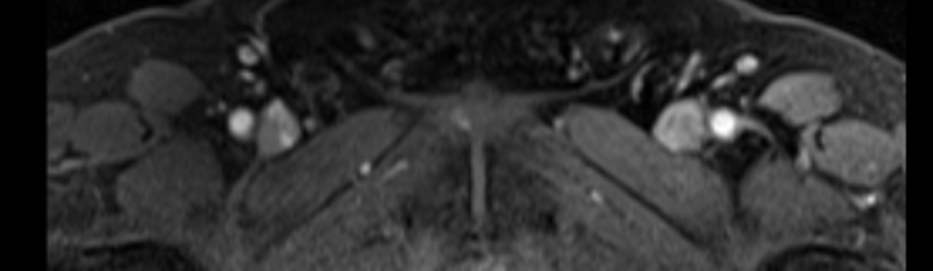
\includegraphics[width=.3\textwidth]{02_methods/figures/original.pdf}} \hfill
  \subfigure[Candidates region after clustering.]{\label{fig:cand}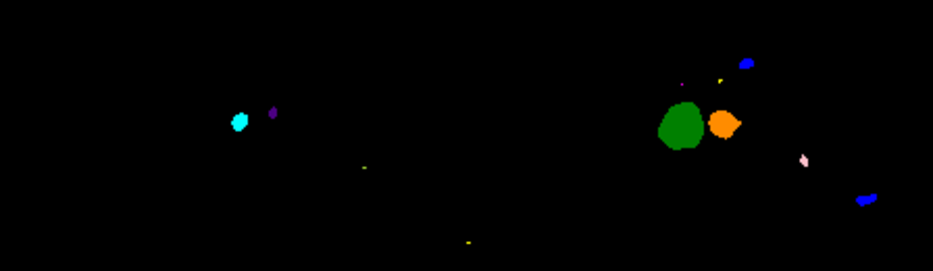
\includegraphics[width=.3\textwidth]{02_methods/figures/candidate.pdf}} \hfill
  \subfigure[Regions selected after applying the different criteria.]{\label{fig:final}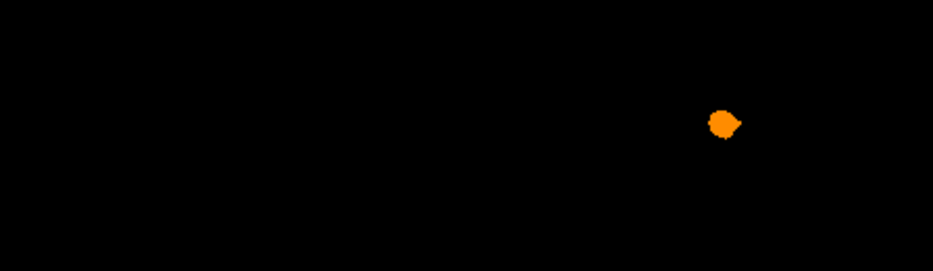
\includegraphics[width=.3\textwidth]{02_methods/figures/aif.pdf}}
  \hspace*{\fill}
  \caption{Illustration of the segmentation of the area used to determine the \acs*{aif}.}
  \label{fig:aif}
\end{figure*}

\begin{description}
  \item[Segmentation of artery voxels and patient-based \ac{aif} estimation] The \ac{aif} signal from \ac{dce}-\ac{mri} can be manually estimated by selecting the most-enhanced voxels from the femoral or iliac arteries~\citep{meng2010comparison}.
    Few methods have been proposed to address the automated extraction
    of the \ac{aif} signal.
    \citeauthor{chen2008automatic} successively filtered the possible
    candidates to be considered as the \ac{aif} such that~\citep{chen2008automatic}:
    (i) dynamic signals with a small peak and voxels with a small wash-in are rejected by thresholding,
    (ii) a blob detector is used and large enough regions are maintained, and
    (iii) circular and cylindricality criteria are used to reject the false positives.
    \citeauthor{zhu2011automated} proposed an iterative method that
    involves the selection of voxels that best fit a gamma variate function~\citep{zhu2011automated}.
    However, this method requires the computation of the first and
    second derivatives as well as the maximum curvature points.
    \citeauthor{shanbhag2012generalized} proposed the following 4-step algorithm~\citep{shanbhag2012generalized,fennessy2015quantitative}:
    (i) remove the slices with artifacts and find the best slices based on intrinsic anatomic landmarks and enhancement characteristics,
    (ii) find the voxel candidates using the maximum enhanced voxels and a multi-label maximum entropy based thresholding algorithm,
    (iii) exclude the region next to the endorectal coil, and
    (iv) select the best 5 candidates that meet the enhancement characteristics and are correlated.

    All the above methods are rather complex, therefore,  we propose a simpler method that is based on the following reasonable assumptions:
    (i) all possible \ac{aif} signal candidates should have a similar shape,
    (ii) they should all have high enhancement, and
    (iii) the arteries should be almost round and within a size range.
    Therefore, each slice is clustered into regions using K-means clustering with $k=6$.
    The cluster made of the most enhanced signals is selected since it contains the artery signals.
    In this regards, the selection criteria corresponds to the 90\textsuperscript{th} percentile of the maximum \ac{dce}-\ac{mri} signal.
    Finally, regions with an eccentricity smaller than $0.5$ and an area in the range of $[100, 400]$ voxels are kept.
    Additionally, to remove voxels contaminated by the partial volume effect, only the $10\%$ most enhanced voxels of the possible candidates are kept as proposed by~\citep{schabel2008uncertainty} and the average signal is computed.
    A summary of the different segmentation steps is presented in Fig.\,\ref{fig:aif}.
    \item[Conversion of \ac{mri} signal intensity to concentration] To estimate the free parameters of the Tofts model (see Eq.\,\eqref{eq:exttofts}), the concentrations $C_t(t)$ and $C_p(t)$ need to be computed from the \ac{mri} signal intensity and the \ac{aif} signal, respectively.
      This conversion is based on the equation of the FLASH sequence\textemdash see~\ref{app:signaltoconc} for details\textemdash and is formulated as in Eq.\,\eqref{eq:conv}:
      \begin{equation}
        c(t) = \frac{1}{TR \cdot r_1} \ln\left( \frac{1 - \cos \alpha \cdot S^{*}\frac{s(t)}{S_0}}{1 - S^{*}\frac{s(t)}{S_0}} \right) - \frac{R_{10}}{r_1} ,
        \label{eq:conv}
      \end{equation}
      \noindent with,
      \begin{equation}
        S^{*} = \frac{1 - \exp(- TR \cdot R_{10})}{1 - \cos \alpha \cdot \exp(- TR \cdot R_{10})} ,
        \label{eq:sstarconv}
      \end{equation}
      \noindent where $s(t)$ is the \ac{mri} signal, $S_0$ is the \ac{mri} signal prior to the injection of the contrast media, $\alpha$ is the flip angle, $TR$ is the \acf{tr}, $R_{10}$ is the pre-contrast tissue relaxation time also equal to $\frac{1}{T_{10}}$, and $r_1$ is the relaxivity coefficient of the contrast agent.

      $T_{10}$ can be estimated from the acquisition of a T$_1$ map.
      However, this modality is not part of the clinical trial in this research and the value of $T_{10}$ is fixed to \SI{1600}{\ms} for both blood and prostate, in accordance with the values found in the literature~\citep{fennessy2015quantitative,de2004mr,carr2011magnetic}.
      \item[Estimation of population-based \ac{aif}] While estimating
        the pharmacokinetic parameters using the Tofts model, the \ac{aif} concentration $C_p(t)$ can be computed either from the patient or a population.
        In the two previous sections, we presented the algorithms that
        allow for the estimation of the patient-based \ac{aif} concentration.
        For a comparison with the previous approach, we also computed a population-based \ac{aif} that will be used later to compare the performance of both approaches.
        In this regard, the population-based \ac{aif} was estimated in
        accordance with the method of~\citep{meng2010comparison} by
        fitting the average patient-based \ac{aif}s to the model
        of~\cite{parker2006experimentally} which is formulated as
        shown in Eq.\,\eqref{eq:parker}, as follows:
        \begin{equation}
          C_p(t) = \sum_{n=1}^{2} \frac{A_n}{\sigma_n \sqrt{2 \pi}} \exp\left(\frac{- (t- T_n)^2}{2\sigma_{n}^{2}}\right) + \frac{\alpha \exp(-\beta t)}{1 + \exp{-s (t - \tau)}} ,
          \label{eq:parker}
        \end{equation}
        \noindent where $A_n$, $T_n$, and $\sigma_n$ are the scaling
        constants, centers, and widths of the n\textsuperscript{th}
        Gaussian, respectively; $\alpha$ and $\beta$ are the amplitude
        and decay constant of the exponential, respectively; and $s$ and $\tau$ are the width and center of the sigmoid function, respectively.
\end{description}

The parameters are estimated by fitting the model using constrained non-linear least-squares optimization, solved with the Trust Region Reflective algorithm~\citep{sorensen1982newton} and bounding the parameters to be positive.

\subsubsection{\acs*{pun} model}\label{sec:pun}

\citeauthor{gliozzi2011phenomenological} showed that the \ac{pun} approach can be used for \ac{dce}-\ac{mri} analysis~\citep{gliozzi2011phenomenological}.
The model has been successfully used in a \ac{cad} system proposed by~\cite{giannini2015fully}.
This model can be expressed as in Eq.\,\eqref{eq:pun}:

\begin{equation}
  s_n(t) = \exp\left[rt + \frac{1}{\beta} \left( a_0 - r \right) \left( \exp(\beta t) - 1 \right) \right],
  \label{eq:pun}
\end{equation}

\noindent with

\begin{equation}
  s_n(t) = \frac{s(t) - S_0}{S_0},
  \label{eq:enh}
\end{equation}

\noindent where $s(t)$ and $S_0$ are the \ac{mri} signal intensity at
time $t$ and the average pre-contrast \ac{mri} signal intensity,
respectively; and $r$, $a_0$, and $\beta$ are the free parameters of the model.

The parameters are estimated by fitting the model using non-linear
least-squares optimization solved with Levenberg-Marquardt algorithm.

\subsubsection{Semi-quantitative analysis}\label{sec:semi}

The semi-quantitative analysis of the \ac{dce}-\ac{mri} is equivalent to extracting curve characteristics directly from the signal without a strict theoretical pharmacokinetic meaning.
In this work, we use the model presented by~\cite{huisman2001accurate}, which formulates the \ac{mri} signal as in Eq.\,\eqref{eq:huisman}:

\begin{equation}
  s(t) = \begin{cases}
    S_0 & 0 \leq t \leq t_0 \\
    S_M - (S_M - S_0) \exp\left( \frac{-(t - t_0)}{\tau} \right) & t_0 < t \leq t_0 + 2 \tau \\
    S_M - (S_M - S_0) \exp\left( \frac{-(t - t_0)}{\tau} \right) + w(t - t_0 + 2 \tau) & t > t_0 + 2 \tau
  \end{cases}
  \label{eq:huisman}
\end{equation}

\noindent where $s(t)$ is the \ac{mri} signal intensity, $S_0$ is the
pre-contrast signal intensity, $t_0$ is the time corresponding to the
start of enhancement, $S_M$ and $\tau$ are the maximum of the signal
and the exponential time constant, respectively, and $w$ is the slope of the linear part.

\citeauthor{huisman2001accurate} argue that curve fitting via
least-squares minimization using the Nelder-Mead algorithm leads to
inaccurate estimations of the parameters free parameters.
Mainly the issue comes from an incorrect estimation of the start of
enhancement $t_0$, leading to an incorrect estimation of the other parameters.
Therefore, \citeauthor{huisman2001accurate} to
(i) robustly estimate $t_0$,
(ii) estimate $S_0$ by averaging the samples between $0$ and $t_0$,
(ii) estimate $w$ depending on whether the slope is significant or
not, and
(iii) estimate $S_M$, which should be the point of intersection of the most probable slope line and the plateau.

Instead of these successive estimations, we propose a unified optimization in which $t_0$ is fixed since it is a key parameter.
Therefore, $t_0$ is robustly estimated from the \ac{aif} signal since this is the most enhanced signal in which the start of enhancement is easily identifiable.
The \ac{aif} signal is computed as discussed in Section~\ref{sec:tofts}.
$t_0$ is estimated by finding the maximum of the first derivative of the \ac{aif} signal, always occurring at the beginning of the signal.
Then, the function in Eq.\,\eqref{eq:huisman} is fitted using non-linear least squares with the Trust Region Reflective algorithm~\citep{sorensen1982newton}.
Furthermore, the parameters $\tau$ and $S_M$ are bounded during the optimization to ensure robust estimations.
$\tau$ is bounded between $t_0$ and $t_f$, which is the time of the
last sample, and $S_M$ is bounded between $S_0$ and $\max(s(t))$.


From Eq.\,\eqref{eq:huisman}, the following features can be extracted:
(i) the wash-in corresponding to the slope between $t_0$ and $t_0 + 2 \tau$,
(ii) the wash-out corresponding to the parameter $w$,
(iii) the area under the curve between $t_0$ and the end of the signal,
(iv) the exponential time constant $\tau$, and
(v) the relative enhancement of $S_M - S_0$.

%%% Local Variables:
%%% mode: latex
%%% TeX-master: "../main"
%%% End:
